\subsection{Android}

\par
Android es un sistema operativo basado en el núcleo Linux. Fue diseñado principalmente para dispositivos móviles con pantalla táctil, como teléfonos inteligentes, tablets o tabléfonos; y también para relojes inteligentes, televisores y automóviles. Inicialmente fue desarrollado por Android Inc. la cual fue fundado en 2003 por Andy Rubin, Rich Miner, Nick Sears y Chris White con el objetivo de desarrollar \textquotedblleft dispositivos móviles que están al corriente de la ubicación y preferencias del usuario \textquotedblright\cite{android-wiki}. En un principio la intención era desarrollar un sistema operativo avanzado para cámaras digitales, pero más tarde se cambió el foco al determinar que el mercado de las cámaras digitales no era lo suficientemente grande. Se redirigirían los esfuerzos a crear un sistema que pudiera competir con Symbian y Windows Mobile\cite{android-xataka}. La versión básica de Android es conocida como Android Open Source Project (AOSP)\cite{android-wiki}. A continuación, una imagen de la evolución del logo de Android. 

\begin{figure}[H]
	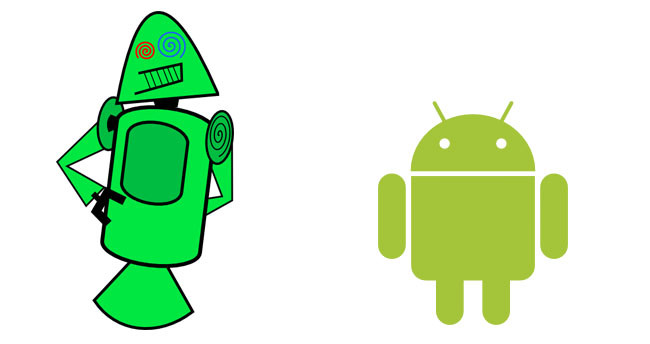
\includegraphics[width=\textwidth]{android1.jpg}
	\caption{Diseño preliminar para el logo de Android (Izquierda) y el logo oficial (Derecha)}
\end{figure}

\par \noindent
A partir del año 2011 Google ha ido actualizando la versión de Android, todos los años. Hoy en día la última versión de Android es \textquotedblleft Android 8.0 Oreo \textquotedblright. Sin embargo, la versión de Android con más dispositivo o smartphones, en uso actualmente, es Android 5.0 Lollipop, la cual será presentada a continuación.

\par \noindent
A continuación se verán las tecnologías que se aplicarón en el área de electrónica.